\section{Redes de Petri}

\subsection{Visión general}

Las redes de Petri (\acrfull{PN}) son una herramienta de modelado gráfico y matemático utilizada para
describir y analizar el comportamiento de los sistemas concurrentes. Fueron introducidas por el
investigador alemán Carl Adam Petri en su tesis doctoral \cite{petri1962} y desde entonces se han aplicado en diversos
campos como la informática, la ingeniería y la biología. Puede encontrar un resumen conciso
de la teoría de las redes de Petri, sus propiedades, análisis y aplicaciones en \cite{murata1989}.

Una red de Petri es un grafo dirigido bipartito formado por un conjunto de lugares, transiciones
y arcos. Hay dos tipos de nodos: lugares y transiciones. Los lugares representan el estado del
sistema, mientras que las transiciones representan eventos o acciones que pueden ocurrir. Los
arcos conectan lugares a transiciones o transiciones a lugares. No puede haber arcos entre
dos lugares o entre dos transiciones, preservando así la propiedad bipartita.

Los lugares pueden contener cero o más marcas o fichas. Los tokens se utilizan para representar la
presencia o ausencia de entidades en el sistema, como recursos, datos o procesos. En la clase
más simple de redes de Petri, los tokens no llevan ninguna información y son indistinguibles
unos de otros. El número de fichas en un lugar o la simple presencia de una ficha es lo que
transmite significado en la red. Las fichas se consumen y se producen al dispararse las
transiciones, lo que da la impresión de que se mueven a través de los arcos.

En la representación gráfica convencional, los lugares se representan mediante círculos,
mientras que las transiciones se representan como rectángulos. Las fichas se representan como
puntos negros dentro de los lugares, como se ve en la Fig. \ref{fig:petri-net-example}.

\begin{figure}[!htb]
      \centering
      \includesvg[width=0.9\linewidth]{petri-net-example.svg}
      \caption{Ejemplo de una red de Petri. \uppercase{PLACE 1} contiene una marca.}
      \label{fig:petri-net-example}
\end{figure}

Cuando una transición se dispara, consume fichas de sus lugares de entrada y produce fichas en
sus lugares de salida, lo que refleja un cambio en el estado del sistema. El disparo de una
transición se activa cuando hay suficientes fichas en sus lugares de entrada.
En la Fig. \ref{fig:petri-net-transition-example},
podemos ver cómo se producen los disparos uno detrás del otro.

\begin{figure}[!htb]
      \centering
      \includesvg[width=0.9\linewidth]{petri-net-transition-example.svg}
      \caption{Ejemplo de disparo de una transición:
            La transición 1 se dispara primero, luego se dispara la transición 2.}
      \label{fig:petri-net-transition-example}
\end{figure}

El disparo de las transiciones habilitadas no es determinista, es decir, se disparan
aleatoriamente mientras estén habilitadas.
Una transición deshabilitada se considera \emph{muerta} si
no hay ningún estado alcanzable en el sistema que pueda llevar a que la transición se habilite.
Si todas las transiciones de la red están muertas, entonces la red también se considera \emph{muerta}.
Este estado es análogo al bloqueo (\textit{deadlock}) de un programa informático.

Las redes de Petri pueden utilizarse para modelar y analizar una amplia gama de sistemas,
desde sistemas sencillos con unos pocos componentes hasta sistemas complejos con muchos
componentes que interactúan entre sí. Pueden utilizarse para detectar problemas posibles en
un sistema, optimizar su rendimiento y diseñar e implementar sistemas de forma más eficaz.

También pueden utilizarse para modelar procesos industriales \cite{aalst1994putting}, para
validar requisitos de software expresados como casos de uso \cite{silva2004applying} o para
especificar y analizar sistemas en tiempo real \cite{kavi1996specification}.

En concreto, las redes de Petri pueden utilizarse para detectar deadlocks en el código fuente
modelando el programa de entrada como una red de Petri y analizando después la estructura de
la red resultante. Se demostrará que este enfoque es formalmente sólido y practicable para el
código fuente escrito en el lenguaje de programación Rust.

\subsection{Modelo matemático formal}

Una red de Petri es un tipo particular de grafo bipartito, con pesos y dirigido, dotado de un
estado inicial denominado \emph{marcado inicial}, $M_0$.
Para este trabajo, se utilizará la siguiente
definición general de una red de Petri tomada de \cite{murata1989}.

\begin{definition}{Petri net}{petri-net}
      Una red de Petri es una 5-tupla, $ PN = (P, T, F, W, M_{0}) $ donde:

      \begin{quote}
            $ P = \{ p_1, p_2, \dots, p_m \} $ es un conjunto finito de lugares,\\
            $ T = \{ t_1, t_2, \dots, t_n \} $ es un conjunto finito de transiciones,\\
            $ F \subseteq (P \times T) \cup (T \times P) $ es un conjunto de arcos (relación de flujo),\\
            $ W: F \leftarrow \{1, 2, 3, ... \} $ es una función de peso para los arcos,\\
            $ M_{0}: P \leftarrow \{0, 1, 2, 3, .... \} $ es el marcado inicial,\\
            $ P \cap T = \varnothing $ y $ P \cup T \neq \varnothing $
      \end{quote}
\end{definition}

En la representación gráfica, los arcos se etiquetan con su peso que es un número entero no
negativo $k$. Normalmente el peso se omite si es igual a 1. Un arco con peso $k$ puede
interpretarse como un conjunto de $k$ arcos paralelos distintos.

Un \emph{marcado (estado)} asocia a cada lugar un número entero no negativo $l$.
Si un marcado asigna al lugar $p$ un número entero no negativo $l$,
decimos que $p$ está \emph{marcado con $l$ marcas o tokens}.
Pictóricamente, denotamos esto colocando $l$ puntos negros (fichas) en el lugar $p$.
El \emph{p-ésimo} componente de $M$, denotado por $M(p)$, es el número de fichas en el lugar $p$.

Una definición alternativa de las redes de Petri utiliza un multiconjunto (\emph{bag}) en lugar de un conjunto para
definir los arcos, permitiendo así la presencia de múltiples elementos. Puede encontrarse en la
literatura, por ejemplo, \cite[Definition 2.3]{peterson1981}.

Como ejemplo, consideremos la red de Petri $ PN_{1} = (P, T, F, W, M) $ donde:

\begin{quote}
      $ P = \{ p_1, p_2 \} $,\\
      $ T = \{ t_1, t_2 \} $,\\
      $ F = \{ (p_1, t_1), (p_2, t_2), (t_1, p_2), (t_2, p_2) \} $,\\
      $ W(a_i) = 1 \quad \forall a_i \in F $\\
      $ M(p_1) = 0, M(p_2) = 0 $
\end{quote}

Esta red no contiene fichas y todos los pesos de los arcos son iguales a 1.
Se muestra en la Fig. \ref{fig:petri-net-formal-example}.

\begin{figure}[!htb]
      \centering
      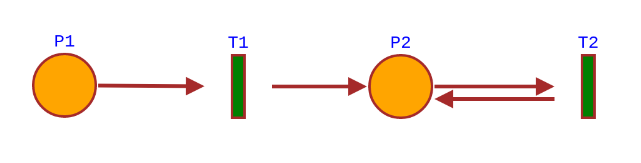
\includegraphics[scale=0.50]{petri-net-formal-example.png}
      \caption{Example of a small Petri net containing a self-loop.}
      \label{fig:petri-net-formal-example}
\end{figure}

La Fig. \ref{fig:petri-net-formal-example}
contiene una estructura interesante que encontraremos más adelante.
Esto motiva la siguiente definición.

\begin{definition}{Bucle}{self-loop}
      Un lugar $p$ y una transición $t$ definen un bucle si
      $p$ es a la vez un lugar de entrada y un lugar de salida de $t$.
\end{definition}

En la mayoría de los casos, nos interesan las redes de Petri que no contienen bucles
las cuales se denominan \emph{puras}.

\begin{definition}{Red de Petri pura}{pure-petri-net}
      Se dice que una red de Petri es pura si no tiene bucles.
\end{definition}

Además, si el peso de cada arco es igual a uno, llamamos a la red de Petri \emph{ordinaria}.

\begin{definition}{Red de Petri ordinaria}{ordinary-petri-net}
      Se dice que una red de Petri es ordinaria si todos los pesos de sus arcos son 1, es decir,
      \begin{equation*}
            W(a) = 1 \quad \forall a \in F
      \end{equation*}
\end{definition}

\subsection{Disparo de transiciones}
\label{sec:transition-firing}

La regla de disparo de transición es el concepto central de las redes de Petri. A pesar de ser
aparentemente simple, sus implicaciones son de gran alcance y complejidad.

\begin{definition}{Regla de disparo de transiciones}{transition-firing-rule}
      Sea $ PN = (P, T, F, W, M_{0}) $ una red de Petri.
      \begin{enumerate}[label=(\roman*)]
            \item Se dice que una transición $t$ está habilitada si cada lugar de entrada $p$ de $t$
                  marcado con al menos $W(p, t)$ marcas
                  donde $W(p,t)$ es el peso del arco que va de $p$ de $t$.
            \item Una transición activada puede dispararse o no, dependiendo de si el evento tiene
                  lugar o no.
            \item El disparo de una transición activada $t$ elimina
                  $W(t,p)$ marcas de cada lugar de entrada $p$ de $t$
                  donde $W(t, p)$ es el peso del arco de $t$ a $p$.
      \end{enumerate}
\end{definition}

Siempre que se habiliten varias transiciones para un marcado $M$ dado, puede dispararse
cualquiera de ellas. La elección es no determinista. Se dice que dos transiciones habilitadas
están en \emph{conflicto} si el disparo de una de ellas inhabilita la otra transición.
En este caso, las transiciones compiten por la ficha colocada en un lugar de entrada compartido.

Si dos transiciones $t_1$ y $t_2$ están habilitadas en algún marcado pero no están en conflicto, pueden
dispararse en cualquier orden, es decir, $t_1$ luego $t_2$ o $t_2$ luego $t_1$.
Tales transiciones representan eventos que pueden ocurrir concurrentemente o en paralelo.
En este sentido, el modelo de red de Petri adopta un modelo de paralelismo basado en el intercalado (\emph{interleaved model of parallelism}),
es decir, el comportamiento del sistema es el resultado de un intercalado arbitrario de los eventos paralelos.

Las transiciones sin lugares de entrada ni lugares de salida reciben un nombre especial.

\begin{definition}{Transición fuente (\textit{Source transition})}{source-transition}
      Una transición sin ningún lugar de entrada se denomina transición fuente.
\end{definition}

\begin{definition}{Transición sumidero (\textit{Sink transition})}{sink-transition}
      Una transición sin lugar de salida se denomina transición de sumidero.
\end{definition}

Cabe destacar que una transición fuente se activa incondicionalmente y produce fichas sin
consumir ninguna, mientras que el disparo de una transición sumidero consume fichas sin
producir ninguna.

\subsection{Simuladores en línea}

Para familiarizarse con la dinámica de las redes de Petri, resulta útil simular algunos ejemplos
en línea, ya que ver una red de Petri en acción es más claro que cualquier explicación estática
sobre el papel. Hemos reunido algunas herramientas con este fin para aliviar la carga del lector.

\begin{itemize}
      \item Puede encontrar un sencillo simulador hecho por Igor Kim en \url{https://petri.hp102.ru/}.
            La herramienta incluye un vídeo tutorial en Youtube y redes de ejemplo.
      \item Como complemento, el profesor Wil van der Aalst de la Universidad de Hamburgo ha
            elaborado una serie de tutoriales interactivos. Estos tutoriales son archivos de Adobe
            Flash Player (con extensión
            \texttt{.swf}) que los navegadores web modernos no pueden ejecutar.
            Por suerte, se puede
            utilizar un emulador Flash en línea como el que se encuentra en \url{https://flashplayer.fullstacks.net/?kind=Flash_Emulator}
            para cargar los archivos
            y ejecutarlos.
      \item Otro editor y simulador de redes de Petri en línea es \url{http://www.biregal.com/}.
            El usuario puede dibujar la red, añadir los tokens y luego disparar manualmente las
            transiciones.
\end{itemize}

\subsection{Ejemplos de modelado}

En esta subsección, se presentan varios ejemplos sencillos para introducir algunos conceptos
básicos de las redes de Petri que son útiles en el modelado. Esta subsección se ha adaptado de
\cite{murata1989}.

Para otros ejemplos de modelado, como el problema de exclusión mutua, los semáforos
propuestos por Edsger W. Dijkstra, el problema del productor/consumidor y el problema de los
filósofos cenando, se remite al lector a \cite[Chap. 3]{peterson1981} y \cite{reisig2013}.

\subsubsection{Máquinas de estado finito}

Las máquinas de estados finitos (\acrfull{FSM}) pueden representarse mediante una subclase de redes de Petri.

Como ejemplo de máquina de estado finito, consideremos una máquina expendedora de café.
Acepta monedas de \EUR{1} o \EUR{2} euros y vende dos tipos de café, el primero cuesta \EUR{3} euros y el
segundo \EUR{4} euros.
Supongamos que la máquina puede contener hasta \EUR{4} y no devuelve ningún cambio.
Entonces, el diagrama de estados
de la máquina puede representarse mediante la red de Petri
que se muestra en la Fig. \ref{fig:state-machine-example}.

\begin{figure}[!htb]
      \centering
      \includesvg[width=\linewidth]{state-machine-example.svg}
      \caption{La red de Petri para una máquina expendedora de café,
            es equivalente a un diagrama de estados.}
      \label{fig:state-machine-example}
\end{figure}

Las transiciones representan la inserción de una moneda del valor etiquetado, por ejemplo,
``Insert \EUR{1} coin''. Los lugares representan un posible estado de la máquina, es
decir, la cantidad de dinero almacenada actualmente en su interior. El lugar situado más a la
izquierda, etiquetado ``\EUR{0}'', está marcado con una ficha y corresponde al estado inicial del
sistema.

Ahora podemos presentar la siguiente definición de esta subclase de redes de Petri.

\begin{definition}{Máquinas de estado}{state-machines}
      Una red de Petri en la que cada transición tiene exactamente un arco entrante y
      exactamente un arco saliente se conoce como máquina de estados.

      Cualquier \acrshort{FSM} (o su diagrama de estados) puede modelarse con una máquina de estados.
\end{definition}

La estructura de un lugar $p_1$ que tiene dos (o más) transiciones de salida $t_1$ y $t_2$ se denomina
conflicto, decisión o elección, según la aplicación en cuestión.
Esto se ve en el lugar inicial de la Fig. \ref{fig:state-machine-example},
donde el usuario debe seleccionar qué moneda introducir al principio.

\subsubsection{Actividades en paralelo}

A diferencia de las máquinas de estados finitos, las redes de Petri también pueden modelar
actividades paralelas o concurrentes.
En la Fig. \ref{fig:parallel-activities-example} se muestra un ejemplo de ello, en el que la
red representa la división de una tarea mayor en dos subtareas que pueden ejecutarse en
paralelo.

\begin{figure}[!htb]
      \centering
      \includesvg[width=0.8\linewidth]{parallel-activities-example.svg}
      \caption{La red de Petri que representa dos actividades paralelas en forma de bifurcación.}
      \label{fig:parallel-activities-example}
\end{figure}

La transición ``Fork'' se disparará antes que ``Task 1'' y ``Task 2'' y que ``Join'' sólo se disparará después
de ambas tareas se completan. Pero tenga en cuenta que el orden en que se ejecutan la ``Task 1'' y
la ``Task 1''  no es determinista. La tarea 1 podría dispararse antes, después o al mismo tiempo
que la tarea 2. Es precisamente esta propiedad de la regla de disparo en las redes de Petri la
que permite modelar sistemas concurrentes.

\begin{definition}{Concurrencia en redes de Petri}{petri-net-concurrency}
      Se dice que dos transiciones son concurrentes si son causalmente independientes, es
      decir, el disparo de una transición no causa ni es provocado por el disparo de la otra.
\end{definition}

Observe que cada lugar de la red de la Fig. \ref{fig:parallel-activities-example}
tiene exactamente un arco entrante y un arco saliente.
Esta subclase de redes de Petri permite representar la concurrencia pero no las
decisiones (conflictos).

\begin{definition}{Grafos marcados (\textit{marked graphs})}{marked-graphs}
      Una red de Petri en la que cada lugar tiene exactamente un arco entrante y exactamente
      un arco saliente se conoce como grafo marcado (\textit{marked graph}).
\end{definition}

\subsubsection{Protocolos de comunicación}

Los protocolos de comunicación también pueden representarse en redes de Petri.
La fig. \ref{fig:communication-protocols-example}
ilustra un protocolo sencillo en el que el Proceso 1 envía mensajes al Proceso 2 y espera a
recibir un acuse de recibo antes de continuar.
Ambos procesos se comunican a través de un
canal con búfer cuya capacidad máxima es de un mensaje.
Por lo tanto, sólo un mensaje puede
estar viajando entre los procesos en un momento dado.
Para simplificar, no se ha incluido ningún mecanismo de \emph{timeout}.

\begin{figure}[!htbp]
      \centering
      \includesvg[width=\linewidth]{communication-protocols-example.svg}
      \caption{Modelo simplificado de red de Petri de un protocolo de comunicación.}
      \label{fig:communication-protocols-example}
\end{figure}

Se podría incorporar al modelo un tiempo de espera máximo para la operación de envío añadiendo una
transición $t_{timeout}$ con aristas de ``Wait for ACK'' a ``Ready to send''.
Esto mapea la decisión entre recibir el acuse de recibo y el tiempo de espera.

\subsubsection{Control de sincronización}

En un sistema multihilo, los recursos y la información se comparten entre varios hilos. Esta
compartición debe controlarse o sincronizarse para garantizar el correcto funcionamiento del
sistema global. Las redes de Petri se han utilizado para modelar diversos mecanismos de
sincronización, incluidos los problemas de exclusión mutua, lectores-escritores y productores-
consumidores \cite{murata1989}.

En la Fig. \ref{fig:readers-writers-example} se muestra una red de Petri para un sistema de lectores-escritores con $k$ procesos.
Cada marca representa un proceso y la elección de T1 o T2 representa si el proceso realiza una
operación de lectura o de escritura.

Utiliza aristas ponderadas para eliminar atómicamente $k - 1$ tokens de P3 antes de realizar una
escritura (transición T2), evitando así que los lectores entren en el bucle derecho de la red.

Como máximo $k$ procesos pueden estar leyendo al mismo tiempo, pero cuando un proceso esté
leyendo, ningún proceso podrá leer, es decir, P2 estará vacío. Se puede comprobar fácilmente
que la propiedad de exclusión mutua se satisface para el sistema.

\begin{figure}[!htbp]
      \centering
      \includesvg[width=\linewidth]{readers-writers-example.svg}
      \caption{Un sistema de redes de Petri con k procesos que leen o escriben.}
      \label{fig:readers-writers-example}
\end{figure}

Hay que señalar que este sistema no está libre de inanición (\textit{starvation}),
ya que no hay garantía de que una operación de escritura vaya a producirse en algún momento.
Por otro lado, el sistema sí está libre de deadlocks.

\subsection{Propiedades importantes}

En esta subsección veremos conceptos fundamentales para el análisis de redes de Petri que
facilitarán la comprensión de las redes que trataremos en el resto del trabajo.

\subsubsection{Alcanzabilidad}
\label{sec:reachability}

La alcanzabilidad es una de las cuestiones más importantes cuando se estudian las propiedades
dinámicas de un sistema. El disparo de transiciones habilitadas provoca cambios en la
ubicación de las marcas. En otras palabras, cambia el marcado $M$. Una secuencia de disparos
crea una secuencia de marcados en la que cada marcado puede denotarse como un vector de
longitud $n$, siendo $n$ el número de lugares de la red de Petri.

Una \emph{secuencia de disparos} u \emph{ocurrencias} se denota por
$ \sigma = M_0\; t_1\; M_1\; t_2\; M_2\; \cdots\; t_l\; M_l$ o simplemente
$ \sigma = t_1\; t_2\; \cdots\; t_l\; $, ya que las marcas
resultantes de cada disparo se derivan de la
regla de disparo de transición descrita en la Sec. \ref{sec:transition-firing}.

\begin{definition}{Alcanzabilidad (\textit{Reachability})}{reachability}
      Decimos que una marca $M$ es alcanzable desde $M_0$ si existe una secuencia de disparo $\sigma$
      tal que $M$ está contenida en $\sigma$.
\end{definition}

El conjunto de todas las marcas posibles alcanzables desde $M_0$ se denota por $R(N, M_0)$ o más
sencillamente $R(M_0)$ cuando la red en cuestión es obvia. Este conjunto se denomina \emph{conjunto de alcanzabilidad}.

Se puede presentar entonces un problema de suma importancia
en la teoría de las redes de Petri, a saber, el \emph{Problema de alcanzabilidad}:
Encontrar si $M_n \in R(M_0, N)$ para una red y un marcado inicial dados.

En algunas aplicaciones, sólo nos interesan los marcados de un subconjunto de lugares y podemos
ignorar los restantes. Esto da lugar a una variación del problema conocida como
\emph{problema de alcanzabilidad del submarcado} (\textit{submarking reachability problem}).

Se ha demostrado que el problema de la alcanzabilidad es decidible \cite{mayr1981}.
Sin embargo, también se ha demostrado que ocupa un espacio exponencial (formalmente, es
EXPSPACE-hard) \cite{lipton1976}. Se han propuesto nuevos métodos para que los algoritmos
sean más eficientes \cite{kungas2005petri}. Recientemente, \cite{czerwinski2020reachability} mejoraron el
límite inferior y demostraron que el problema no es ELEMENTARY. Estos resultados ponen de
relieve que el problema de la alcanzabilidad sigue siendo un área activa de investigación en
teória de la computación.

Para éste y otros problemas clave, los resultados teóricos más importantes obtenidos hasta
1998 se detallan en \cite{esparza1994decidability}.

\subsubsection{Acotamiento y seguridad}

Durante la ejecución de una red de Petri, los tokens pueden acumularse en algunos lugares.
Diversas aplicaciones sulen necesitar garantizar que el número de fichas en un lugar determinado no supere
una cierta tolerancia. Por ejemplo, si un lugar representa un búfer, nos interesa que el búfer
nunca se desborde.

\begin{definition}{Acotamiento (\textit{Boundedness})}{boundedness}
      Un lugar de una red de Petri es k-acotada o es k-seguro si el número de fichas
      de ese lugar no puede superar un número entero finito $k$ para cualquier marcado
      alcanzable desde $M_0$.

      Una red de Petri es k-acotada o simplemente acotada si todos los lugares están acotados.
\end{definition}

La seguridad es un caso especial de la acotación.
Aplica cuando el lugar contiene 1 ó 0 fichas durante la ejecución.

\begin{definition}{Seguridad (\textit{Safeness})}{safeness}
      Un lugar de una red de Petri es seguro si el número de fichas de ese lugar nunca es
      superior a uno.

      Una red de Petri es segura si cada lugar de esa red es seguro.
\end{definition}

Las redes de las Fig. \ref{fig:state-machine-example}, \ref{fig:parallel-activities-example}
y \ref{fig:communication-protocols-example} son todas seguras.

La red de la Fig. \ref{fig:readers-writers-example} es k-acotada porque todos sus lugares son k-acotados.

\subsubsection{Liveness}

El concepto de liveness es análogo a la ausencia total de deadlocks en los programas informáticos.

\begin{definition}{Liveness}{liveness}
      Se dice que una red Patri $(N, M_0)$ está viva (o equivalentemente se dice que $M_0$ es una
      marca viva (\textit{live}) para $N$) si, para cada marca alcanzable desde $M_0$, es posible disparar
      cualquier transición de la red progresando a través de alguna secuencia de disparo.
\end{definition}

Cuando una red está viva, siempre puede seguir ejecutándose, sin importar las transiciones que
se dispararon antes. Eventualmente, cada transición puede dispararse de nuevo. Si una
transición sólo puede dispararse una vez y no hay forma de volver a activarla, entonces la red
no es viva (\textit{live}).

Esto equivale a decir que la red de Petri está \emph{libre de bloqueo} (\textit{deadlock-free}).
Definamos ahora lo que constituye un bloqueo/deadlock y mostremos ejemplos de ello.

\begin{definition}{Bloqueo en redes de Petri}{petri-net-deadlock}
      Un bloqueo o \textit{deadlock} en una red Patri es una transición (o un conjunto de transiciones) que
      no puede dispararse para ninguna marca alcanzable desde $M_0$. La transición (o un
      conjunto de transiciones) no puede volver a activarse después de un cierto punto de la
      ejecución.
\end{definition}

Una transición está \emph{viva} si no está bloqueada.
Si una transición está viva, siempre es posible
elegir una serie de disparos de transiciones adecuada
para pasar del marcado actual a un marcado que habilite la transición.

Las redes de las Fig. \ref{fig:state-machine-example}, \ref{fig:parallel-activities-example}
and \ref{fig:communication-protocols-example} están todas vivas.
En todos estos casos, después de algunos disparos,
la red vuelve al estado inicial y puede reiniciar el ciclo.

La red de la Fig. \ref{fig:petri-net-example} no está viva.
Después de dos disparos termina de ejecutarse y no puede
ocurrir nada más.
La red de la Fig. \ref{fig:petri-net-formal-example} tampoco está viva,
porque T1 sólo se ejecutará una vez y a partir de ese momento sólo se podrá activar T2.

\subsection{Análisis de alcanzabilidad}

Tras haber introducido el conjunto de alcanzabilidad $R(N, M_0)$ en la Sec. \ref{sec:reachability},
ahora podemos presentar una técnica de análisis importante para las redes de Petri: \emph{el árbol de
      alcanzabilidad} (\textit{reachability tree}).

Ejecutaremos paso a paso el algoritmo para construir el árbol de alcanzabilidad y, a
continuación, presentaremos sus ventajas e inconvenientes. En términos generales, el árbol de
alcanzabilidad tiene la siguiente estructura: Los nodos representan las marcas generadas a partir
de $M_0$, la raíz del árbol y sus sucesores.
Cada arco representa un disparo de transición que transforma un marcado en otro.

\begin{figure}[!htb]
      \centering
      \includesvg[width=0.5\linewidth]{reachability-tree-example.svg}
      \caption{Una red de Petri marcada para ilustrar la construcción de un árbol de alcanzabilidad.}
      \label{fig:reachability-tree-example}
\end{figure}

Considere la red de Petri mostrada en la Fig. \ref{fig:reachability-tree-example}.
La marca inicial es $(1, 0, 0)$.
En este marcado inicial se habilitan dos transiciones: T1 y T3.
Dado que queremos obtener todo el conjunto de alcanzabilidad,
definimos un nuevo nodo en el árbol de alcanzabilidad para cada
marcado alcanzable, que resulta de disparar cada transición. Un arco, etiquetado por la
transición disparada, conduce desde la marca inicial (la raíz del árbol) hasta cada una de las
nuevas marcas. Tras este primer paso (Fig. \ref{fig:reachability-tree-step-1}),
el árbol contiene todas las marcas que son inmediatamente alcanzables desde la marca inicial.

\begin{figure}[!htb]
      \centering
      \includesvg[width=0.5\linewidth]{reachability-tree-step-1.svg}
      \caption{Primer paso para construir el árbol de alcanzabilidad
            de la red de Petri de la Fig. \ref{fig:reachability-tree-example}.}
      \label{fig:reachability-tree-step-1}
\end{figure}

Ahora debemos considerar todas las marcas alcanzables desde las hojas del árbol.

A partir del marcado $(0,0,1)$ no podemos disparar ninguna transición. Esto se conoce como un
\emph{marcado muerto} (\textit{dead marking}).
En otras palabras se trata de un nodo ``sin salida''.
Esta clase de estados finales es especialmente relevante para el análisis de bloqueos.

A partir de la marca de la derecha del árbol, denotada $(1, 1, 0)$, podemos disparar T1 o T3.
Si disparamos T1, obtenemos $(0, 1, 1)$ y si dispara T3, la marca resultante es $(1, 2, 0)$.
Esto produce el árbol de la Fig. \ref{fig:reachability-tree-step-2}.

\begin{figure}[!htb]
      \centering
      \includesvg[width=0.7\linewidth]{reachability-tree-step-2.svg}
      \caption{Segundo paso en la construcción del árbol de alcanzabilidad
            de la red de Petri de la Fig. \ref{fig:reachability-tree-example}.}
      \label{fig:reachability-tree-step-2}
\end{figure}

Observe que partiendo de la marca $(0, 1, 1)$, sólo se habilita la transición T2 que conducirá a una
marca $(0, 0, 1)$ ya vista anteriormente.
Si en cambio tomamos $(1, 2, 0)$ tenemos de nuevo las
mismas posibilidades que partiendo de $(1, 1, 0)$.
Es fácil ver que el árbol seguirá creciendo por ese
camino. Por tanto, el árbol es infinito y
esto se debe a que la red de la Fig. \ref{fig:reachability-tree-example} no está acotada.
Veáse en la Fig. \ref{fig:reachability-tree-final-step} el resultado final abreviado.

\begin{figure}[!htb]
      \centering
      \includesvg[width=\linewidth]{reachability-tree-final-step.svg}
      \caption{El árbol de alcanzabilidad infinita para
            la red de Petri de la Fig. \ref{fig:reachability-tree-example}.}
      \label{fig:reachability-tree-final-step}
\end{figure}

El método presentado anteriormente enumera los elementos del conjunto de alcanzabilidad.
Se producirá cada marca del conjunto de alcanzabilidad y, por tanto, para cualquier red de Petri
con un conjunto de alcanzabilidad infinito, es decir, un número infinito de estados posibles, el
árbol correspondiente también sería infinito.
Sin embargo, lo contrario no es cierto. Una red de
Petri con un conjunto de alcanzabilidad finito puede tener un árbol infinito
(véase la Fig. \ref{fig:reachability-tree-bounded-net-counterexample}).
Esta red es incluso \emph{segura}.
En conclusión, tratar con una red acotada o segura no
es garantía de que el número total de estados alcanzables sea finito.

\begin{figure}[!htb]
      \centering
      \includesvg[width=0.9\linewidth]{reachability-tree-bounded-net-counterexample.svg}
      \caption{Una red de Petri simple con un árbol de alcanzabilidad infinito.}
      \label{fig:reachability-tree-bounded-net-counterexample}
\end{figure}

Para que el árbol de alcanzabilidad sea una herramienta de análisis útil, es necesario idear un
método que lo limite a un tamaño finito. Esto implica en general una cierta pérdida de
información, ya que el método tendrá que mapear (o mejor dicho reducir)
un número infinito de marcados alcanzables a un solo elemento.
La reducción a una representación finita puede lograrse por los siguientes medios.

Observe por un lado que podemos encontrarnos con nodos duplicados en nuestro árbol y que
siempre los tratamos ingenuamente como nuevos. Esto se ilustra más claramente en la Fig.
\ref{fig:reachability-tree-bounded-net-counterexample}.
Por tanto, es posible detener la exploración de los sucesores de un nodo duplicado.

Nótese, por otro lado, que algunas marcados son estrictamente diferentes de las marcas vistas
anteriormente pero permiten el mismo conjunto de transiciones. Decimos en este caso que la
marca con fichas adicionales \emph{cubre} (\textit{covers}) la que tiene el número mínimo de fichas necesarias para
permitir el conjunto de transiciones en cuestión.
Disparar algunas transiciones puede permitirnos acumular un número arbitrario de fichas en un lugar.
Por ejemplo, disparar T3 en la red de Petri que se ve en la
Fig. \ref{fig:reachability-tree-example} muestra exactamente este comportamiento.
En conclusión, bastaría con marcar el lugar de acumulación con una etiqueta especial $\omega$, que significa infinito,
ya que podríamos obtener tantas marcas como quisiéramos en ese lugar.

Por ejemplo, el resultado de convertir el árbol de la Fig. \ref{fig:reachability-tree-final-step}
en un árbol finito se muestra en la Fig. \ref{fig:reachability-tree-final-step-finite}.

\begin{figure}[!htb]
      \centering
      \includesvg[width=0.7\linewidth]{reachability-tree-final-step-finite.svg}
      \caption{El árbol de alcanzabilidad finito para
            la red de Petri de la Fig. \ref{fig:reachability-tree-example}.}
      \label{fig:reachability-tree-final-step-finite}
\end{figure}

Para más detalles sobre

\begin{enumerate}
      \item la técnica de representación de árboles de alcanzabilidad infinita mediante $\omega$,
      \item una definición del algoritmo y los pasos precisos para construir el árbol de alcanzabilidad,
      \item la demostración matemática de que el árbol de alcanzabilidad generado por el algoritmo es finito,
      \item y la distinción entre el árbol de alcanzabilidad y el \emph{grafo de alcanzabilidad} (\textit{reachability graph})
\end{enumerate}

se remite al lector a \cite{murata1989} y \cite{peterson1981}.
Estos conceptos están fuera del alcance de este trabajo y
no son necesarios en los capítulos siguientes.